
%%% Local Variables:
%%% mode: LaTeX
%%% TeX-master: t
%%% End:
\documentclass[paper=letter, fontsize=11pt]{scrartcl} % Standard US Letter paper

\usepackage[T1]{fontenc} % Use 8-bit encoding that has 256 glyphs
\usepackage[english]{babel} % English language/hyphenation
\usepackage{amsmath,amsfonts,amsthm} % Math packages
\usepackage{graphicx} % Images
\graphicspath{{images/}}

% Custom headers and footers
\usepackage[automark,headsepline,footsepline]{scrlayer-scrpage}
\clearpairofpagestyles
\pagestyle{scrheadings}
\ofoot{\pagemark}
\setlength{\headheight}{13.6pt}

% Margins
\usepackage[margin=1in]{geometry}

\numberwithin{equation}{section} 
\numberwithin{figure}{section}   
\numberwithin{table}{section}    

\setlength\parindent{0pt} 
\setlength{\parskip}{1em} 

% Change subsection numbering from 1.1 to "1 a)"
%\renewcommand{\thesubsection}{\thesection\ \alph{subsection})}

%----------------------------------------------------------------------------------------
%   TITLE SECTION
%----------------------------------------------------------------------------------------

\newcommand{\horrule}[1]{\rule{\linewidth}{#1}} 

\title{ 
\normalfont \normalsize 
\textsc{University of North Carolina at Charlotte, Intro to Machine Learning} \\ [25pt] 
\horrule{0.5pt} \\[0.4cm] 
\huge Homework 1 \\ 
\horrule{2pt} \\[0.5cm] 
}

\author{Jordan Mckoy \and Miguel Diaz-Alvarez  \and AJ Carroll}
\date{\normalsize\today} 

\begin{document}

\maketitle 

%----------------------------------------------------------------------------------------
%   PROBLEM 1
%----------------------------------------------------------------------------------------

\section{Overview}
In this project, we were tasked with using the breast 
cancer dataset to implement and evaluate at least five classifiers 
from the following list:
\begin{itemize}
    \item Logistic Regression
    \item Naive Bayes
    \item Perceptron
    \item Support Vector Machine
    \item Decision Tree Classifier
    \item K-Nearest Neighbors
\end{itemize} 
% An example of how to include images. Save image to image folder and replace 
% ImageName with the name of your image
% \begin{center}
%     \includegraphics[width=0.7\textwidth]{ImageName.png}
%     \par\small Caption goes here 
% \end{center}

\section{Preprocessing}
In the processing step, we split the data into 80 percent training and 20 percent testing. 
When splitting data, we set the stratify parameter to yes. This feature ensures that, in each 
split, classes that are rare, such as a positive cancer diagnosis, occur with the same frequency 
as in the main data set. We also opted to test different scalers (MinMax, Standard, no scaler). 
We did this by using Pipeline and GridSearchCV to test multiple different parameters at once. 

\section{Helper Functions}
We used three helper functions in our notebook: \texttt{evaluate}, \texttt{summarize\_grid}, and \texttt{weighted\_recall}.
The ``\texttt{evaluate}'' function takes the model and its name as input parameters. The function trains, tests, displays the confusion matrix, 
prints the classification report, and returns the model metrics. The ``\texttt{summarize\_grid}'' function is used to compare different scalers. 
One of the questions asked how different scaling methods affect different algorithms; this function allows us to take a closer look at this.  
The ``\texttt{weighted\_recall}'' function takes model predictions, true values, the weights of malignant and benign recall, 
and the weight of benign recall as input parameters. This function then computes a ``weighted recall.'' 
Since this is a medical context, we decided to emphasize false negatives, as they can lead to patients being left untreated. 
But if we only focused on that, that model would then diagnose more people with cancer to ensure no one is missed. 
To fix this, we used a portion of the malignant and benign recall scores from a default 60--40 split to obtain a more balanced model. 
This weighted recall metric was used to select the best model.

\section{Naive Bayes}
\begin{center}
    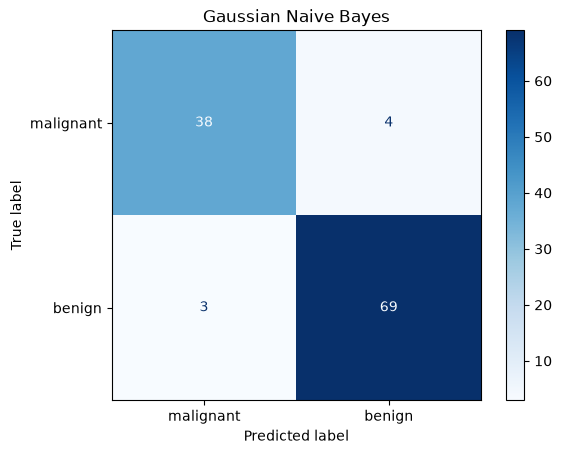
\includegraphics[width=0.7\textwidth]{Bayes.png}
    \par\small Confusion matrix for Naive Bayes model. 
\end{center}

\section{Logistic Regression}
\begin{center}
    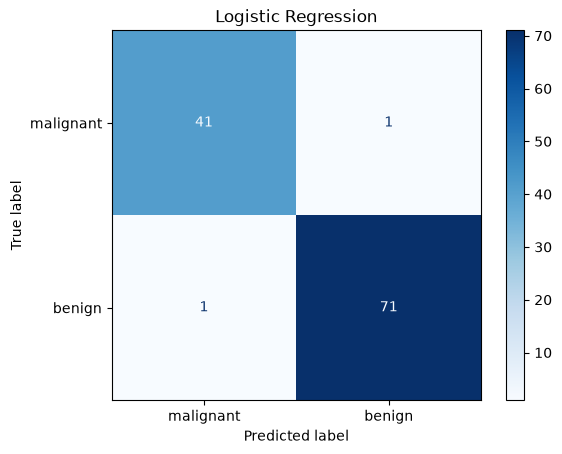
\includegraphics[width=0.7\textwidth]{Log.png}
    \par\small Confusion matrix for Logistic Regression model.
\end{center}

\section{Perceptron}
\begin{center}
    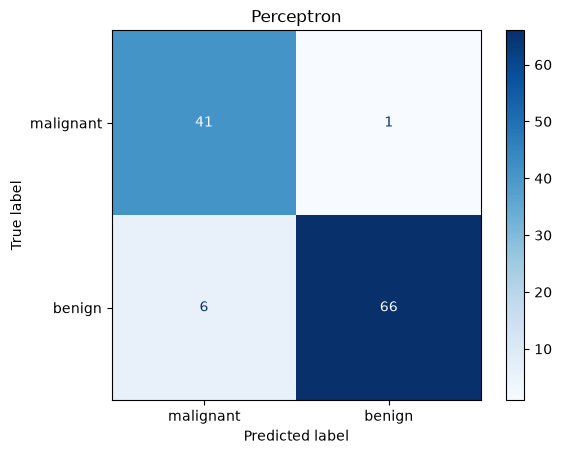
\includegraphics[width=0.7\textwidth]{Per.png}
    \par\small Confusion matrix for Perceptron model.
\end{center}

\section{Support Vector Machine}
\begin{center}
    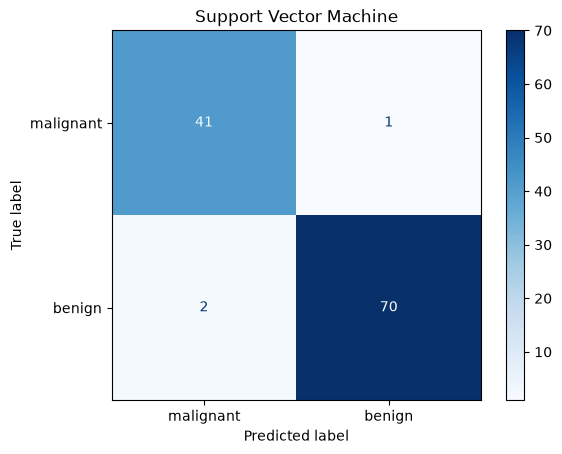
\includegraphics[width=0.7\textwidth]{SVM.png}
    \par\small Confusion matrix for Support Vector Machine model.
\end{center}

\section{Decision Tree Classifier}
\begin{center}
    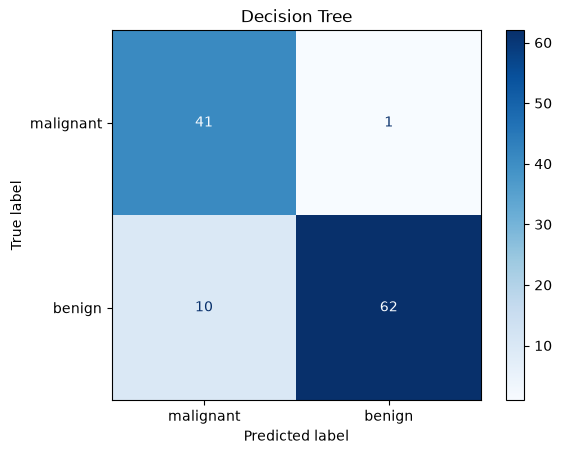
\includegraphics[width=0.7\textwidth]{DT.png}
    \par\small Confusion matrix for Decision Tree Classifier model.
\end{center}

\section{K-Nearest Neighbors}
\begin{center}
    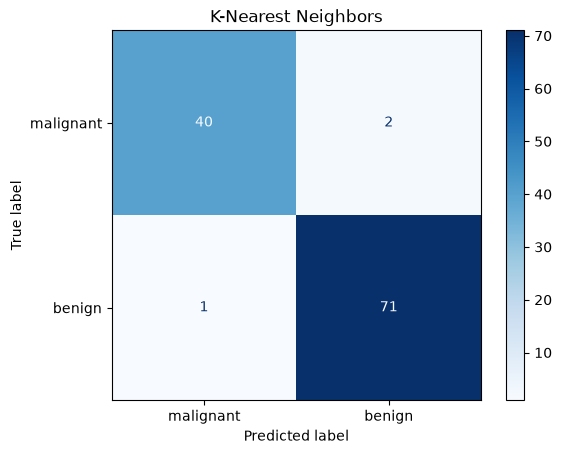
\includegraphics[width=0.7\textwidth]{KNN.png}
    \par\small Confusion matrix for K-Nearest Neighbors model.
\end{center}

\end{document}